%!TEX program = xelatex
% Final oral presentation slides (English version, ~40 min)
% Focus: LWE and Ring-LWE; six preliminary slides; closing 5 min on applications & open problems
\documentclass[aspectratio=169, 11pt]{beamer}

\usepackage{fontspec}
\usepackage{xeCJK}
\setCJKmainfont{Microsoft JhengHei}
\setmainfont{Times New Roman}

\usepackage{amsmath}
\usepackage{amssymb}
\usepackage{tikz}
\usetikzlibrary{calc, arrows.meta}

% -- Colors and theme ---------------------------------------
\definecolor{accent}{RGB}{30, 80, 160}
\definecolor{accentlt}{RGB}{237, 246, 255}
\definecolor{warn}{RGB}{200, 90, 30}

\usetheme{default}
\setbeamercolor{structure}{fg=accent}
\setbeamercolor{title}{fg=accent}
\setbeamercolor{frametitle}{fg=white, bg=accent}
\setbeamercolor{block title}{fg=white, bg=accent}
\setbeamercolor{block body}{bg=accentlt}
\setbeamercolor{itemize item}{fg=accent}
\setbeamercolor{itemize subitem}{fg=accent}
\setbeamertemplate{navigation symbols}{}
\setbeamertemplate{itemize items}[circle]
\setbeamerfont{frametitle}{series=\bfseries}
\setbeamerfont{title}{series=\bfseries}

% frametitle bar with time tag
\setbeamertemplate{frametitle}{%
  \nointerlineskip
  \begin{beamercolorbox}[wd=\paperwidth, ht=2.6ex, dp=1.0ex, leftskip=0.6em, rightskip=0.6em]{frametitle}%
    \bfseries\insertframetitle\hfill{\small\normalfont\insertframesubtitle}%
  \end{beamercolorbox}%
}

% footline: author | section | page
\setbeamertemplate{footline}{%
  \leavevmode\hbox{%
    \begin{beamercolorbox}[wd=.34\paperwidth, ht=2.4ex, dp=1ex, leftskip=.6em]{author in head/foot}%
      \tiny Chung-Chin Huang · L16141149%
    \end{beamercolorbox}%
    \begin{beamercolorbox}[wd=.46\paperwidth, ht=2.4ex, dp=1ex, center]{title in head/foot}%
      \tiny\insertsectionhead%
    \end{beamercolorbox}%
    \begin{beamercolorbox}[wd=.20\paperwidth, ht=2.4ex, dp=1ex, rightskip=.6em]{date in head/foot}%
      \hfill\tiny\insertframenumber\,/\,\inserttotalframenumber%
    \end{beamercolorbox}}%
}

\newcommand{\timetag}[1]{{\small\color{accentlt!50!white}\textbf{[#1]}}}
\newcommand{\R}{\mathbb{R}}
\newcommand{\Z}{\mathbb{Z}}
\newcommand{\Q}{\mathbb{Q}}
\newcommand{\F}{\mathbb{F}}
\newcommand{\OK}{\mathcal{O}_K}
\newcommand{\Tr}{\mathrm{Tr}}
\newcommand{\vol}{\mathrm{vol}}

\title{LWE and Ring-LWE}
\subtitle{The Number-Theoretic Structure of Ideal-Lattice Cryptography --- Final Oral Report (\textasciitilde 40 min)}
\author{Chung-Chin Huang · L16141149}
\institute{Number Theory I · Spring 2026 · National Cheng Kung University}
\date{}

\begin{document}

% ==========================================================
\begin{frame}[plain]
  \titlepage
  \begin{center}\small\color{gray}
    Geometry of numbers $\to$ cyclotomic fields \& ideal lattices $\to$ \textbf{LWE / Ring-LWE} $\to$ post-quantum standards
  \end{center}
\end{frame}

\begin{frame}{Outline}{Time budget $\approx$ 40 min}
  \begin{columns}[T]
    \begin{column}{0.5\textwidth}
      \textbf{Part 0 --- Preliminaries} \timetag{$\sim$10 min}
      \begin{itemize}
        \item Lattice
        \item Minkowski's first theorem
        \item Cyclotomic field
        \item Ideal-lattice structure
        \item Shortest Vector Problem (SVP)
        \item Closest Vector Problem (CVP)
      \end{itemize}
    \end{column}
    \begin{column}{0.5\textwidth}
      \textbf{Part 1 --- LWE} (core) \timetag{$\sim$12 min}\\[-2pt]
      \begin{itemize}\small
        \item Setup; decision vs.\ search versions
        \item Lattice connection; security reduction
        \item Hardness and efficiency bottleneck
      \end{itemize}
      \vspace{4pt}
      \textbf{Part 2 --- Ring-LWE} (core) \timetag{$\sim$13 min}\\[-2pt]
      \begin{itemize}\small
        \item Cyclotomic-ring setup; prime-ideal splitting
        \item Fast NTT multiplication; dual-lattice error
        \item Sample construction and reduction chain
      \end{itemize}
      \vspace{4pt}
      \textbf{Part 3 --- Applications \& open problems} \timetag{$\sim$5 min}
    \end{column}
  \end{columns}
\end{frame}

% ==========================================================
\section{Part 0 --- Preliminaries}

% -- Lattice --
\begin{frame}{Lattice}{Part 0 · Preliminaries 1/6}
  \begin{block}{Definition}
    Take $n$ linearly independent vectors $b_1,\dots,b_n$ in $\R^n$; their integer linear combinations
    \[
      \mathcal{L}=\sum_{i=1}^n \Z\, b_i \subset \R^n
    \]
    form a \textbf{lattice} of rank $n$. The quantity $\det(\mathcal{L}):=|\det B|$ of the basis matrix
    $B=[b_1|\cdots|b_n]$ is the \textbf{covolume}, independent of the chosen basis, and geometrically
    equals the volume of the fundamental domain $\mathcal{F}=B[0,1)^n$.
  \end{block}
  \begin{columns}[c]
    \begin{column}{0.62\textwidth}
      \begin{itemize}\small
        \item One lattice has infinitely many bases; the gap between a ``good'' basis (short, nearly orthogonal) and a ``bad'' one is the source of hard problems.
        \item The smaller the covolume, the denser the lattice points.
        \item Next: an ideal in a number field $\mapsto$ a lattice (ideal lattice), moving algebra into geometry.
      \end{itemize}
    \end{column}
    \begin{column}{0.36\textwidth}
      \centering
      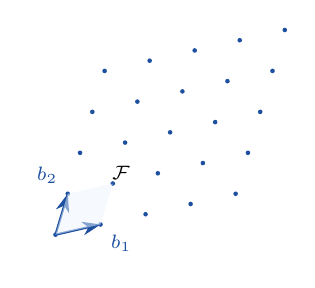
\begin{tikzpicture}[scale=0.52]
        \foreach \i in {0,...,4}\foreach \j in {0,...,4}
          \fill[accent] ($\i*(1.1,0.25)+\j*(0.3,1.0)$) circle (1.6pt);
        \draw[-{Stealth}, accent, thick] (0,0)--(1.1,0.25) node[below right]{\scriptsize$b_1$};
        \draw[-{Stealth}, accent, thick] (0,0)--(0.3,1.0) node[above left]{\scriptsize$b_2$};
        \fill[accentlt, opacity=0.5] (0,0)--(1.1,0.25)--(1.4,1.25)--(0.3,1.0)--cycle;
        \node[font=\scriptsize] at (1.6,1.5) {$\mathcal{F}$};
      \end{tikzpicture}
    \end{column}
  \end{columns}
\end{frame}

% -- Minkowski --
\begin{frame}{Minkowski's First Theorem (1896)}{Part 0 · Preliminaries 2/6}
  \begin{block}{Theorem}
    Let $\mathcal{L}\subset\R^n$ be a lattice and $S\subset\R^n$ a \textbf{centrally symmetric convex body}
    ($x\in S\Rightarrow -x\in S$; bounded, closed, convex). If
    \[
      \vol(S) > 2^n \det(\mathcal{L}),
    \]
    then $S$ contains at least one nonzero lattice point $v\in\mathcal{L}\setminus\{0\}$.
  \end{block}
  \begin{itemize}\small
    \item \textbf{Proof idea}: apply Blichfeldt's pigeonhole argument to $\tfrac12 S$;
      $\vol(\tfrac12 S)>\det(\mathcal{L})$ forces two translated copies to overlap, then
      central symmetry $+$ convexity pull the difference vector back into $S$.
    \item \textbf{Key message}: ``large enough volume $\Rightarrow$ a nonzero lattice point must exist'' ---
      a \textbf{non-constructive} existence theorem: it guarantees a short vector \emph{exists} but gives no way to find it.
    \item This is precisely the geometric root of the hardness of SVP and the foundation of lattice-based security.
  \end{itemize}
\end{frame}

% -- Cyclotomic field --
\begin{frame}{Cyclotomic Field}{Part 0 · Preliminaries 3/6}
  \begin{block}{Setup (take $n=2^k$, power-of-two cyclotomic ring)}
    $\zeta=\zeta_{2n}=e^{i\pi/n}$ is a primitive $2n$-th root of unity; the cyclotomic polynomial is
    $\Phi_{2n}(x)=x^n+1$ (irreducible over $\Q$ when $n=2^k$),
    $K=\Q(\zeta)$, $[K:\Q]=n$.
  \end{block}
  \begin{itemize}\small
    \item The ring of integers $\OK=\Z[\zeta]\cong\Z[x]/(x^n+1)$ is a \textbf{Dedekind domain}
      (Noetherian, integrally closed, every nonzero prime ideal maximal) $\Rightarrow$ unique factorization of every nonzero ideal into prime ideals.
    \item The \textbf{canonical embedding} $\sigma_j(\zeta)=\zeta^{2j-1}$ ($j=1,\dots,n$) gives
      $\sigma:K\hookrightarrow\mathbb{C}^n$; conjugate symmetry places the image in $H\cong\R^n$,
      and it is compatible with ring multiplication (component-wise).
    \item Discriminant: $|\Delta_K|=(2n)^n/2^n=n^n$.
    \item Why $x^n+1$: cleanest irreducibility; $x^n\equiv-1$ gives ``negacyclic convolution''; friendly to the NTT.
  \end{itemize}
\end{frame}

% -- Ideal lattice --
\begin{frame}{Ideal-Lattice Structure}{Part 0 · Preliminaries 4/6}
  \begin{block}{Ideal $\xrightarrow{\ \sigma\ }$ lattice}
    A fractional ideal $\mathfrak{a}\subset\OK$ maps under the canonical embedding to $\sigma(\mathfrak{a})\subset H$,
    a rank-$n$ lattice closed under multiplication by $\OK$ (hence an \textbf{ideal lattice}).
  \end{block}
  \begin{itemize}\small
    \item Exact relation between covolume and ideal norm $N(\mathfrak{a})=[\OK:\mathfrak{a}]$:
      \[
        \det\bigl(\sigma(\OK)\bigr)=\sqrt{|\Delta_K|}=n^{n/2},
        \qquad
        \det\bigl(\sigma(\mathfrak{a})\bigr)=N(\mathfrak{a})\cdot n^{n/2}.
      \]
    \item \textbf{Meaning}: it binds the (arithmetic) ``ideal norm'' to the (geometric) ``lattice volume'';
      ideal multiplication $\leftrightarrow$ an algebraic action on the lattice.
    \item An ideal lattice is a special case of a general lattice, but carries extra ring structure $\Rightarrow$
      \alert{the source of efficiency} (Ring-LWE) and also \alert{the source of security debate} (is ideal-SVP easier?).
  \end{itemize}
\end{frame}

% -- SVP --
\begin{frame}{Shortest Vector Problem (SVP)}{Part 0 · Preliminaries 5/6}
  \begin{columns}[T]
    \begin{column}{0.62\textwidth}
      \begin{block}{Problem}
        Given a (bad) basis of a lattice $\mathcal{L}$, find the length of the shortest nonzero vector
        $\lambda_1(\mathcal{L})=\min_{v\in\mathcal{L}\setminus\{0\}}\|v\|$, or such a $v$.
      \end{block}
      \begin{itemize}\small
        \item \textbf{Approximate SVP$_\gamma$}: find $v\neq0$ with $\|v\|\le\gamma\cdot\lambda_1$.
        \item NP-hard (under randomized reductions, $\gamma=O(1)$); best algorithms run in $2^{\Theta(n)}$.
        \item Best quantum algorithm $2^{0.265n}$ (Laarhoven 2015) $\Rightarrow$ still hard post-quantum.
        \item The security of LWE/Ring-LWE ultimately reduces to this (worst case).
      \end{itemize}
    \end{column}
    \begin{column}{0.36\textwidth}
      \centering
      \begin{tikzpicture}[scale=0.5]
        \foreach \i in {-1,...,3}\foreach \j in {-1,...,3}
          \fill[gray!60] ($\i*(1.2,0.3)+\j*(0.4,1.1)$) circle (1.4pt);
        \draw[-{Stealth}, warn, very thick] (0,0)--(0.4,1.1);
        \node[warn, font=\scriptsize] at (1.2,1.0) {shortest $v$};
      \end{tikzpicture}
      \\[2pt]{\scriptsize find the shortest nonzero lattice point}
    \end{column}
  \end{columns}
\end{frame}

% -- CVP --
\begin{frame}{Closest Vector Problem (CVP)}{Part 0 · Preliminaries 6/6}
  \begin{columns}[T]
    \begin{column}{0.62\textwidth}
      \begin{block}{Problem}
        Given a lattice $\mathcal{L}$ and a target point $t\in\R^n$ (not necessarily on the lattice),
        find the nearest lattice point $v\in\mathcal{L}$ minimizing $\|t-v\|$.
      \end{block}
      \begin{itemize}\small
        \item Generally harder than SVP (SVP $\le$ CVP by reduction).
        \item \textbf{BDD (Bounded Distance Decoding)}: a special case of CVP where $t$ is known to lie
          very close to some lattice point ($<\lambda_1/2$); recover it $\Rightarrow$ unique solution.
        \item \alert{LWE is essentially BDD}: in $b=As+e$, $As$ is a lattice point and $e$ a small error,
          so recovering $s$ $=$ solving BDD on a $q$-ary lattice.
      \end{itemize}
    \end{column}
    \begin{column}{0.36\textwidth}
      \centering
      \begin{tikzpicture}[scale=0.5]
        \foreach \i in {-1,...,3}\foreach \j in {-1,...,3}
          \fill[gray!60] ($\i*(1.2,0.3)+\j*(0.4,1.1)$) circle (1.4pt);
        \coordinate (t) at (1.7,1.6);
        \coordinate (v) at (1.6,1.4);
        \fill[warn] (t) circle (2pt) node[right, font=\scriptsize]{$t$};
        \draw[warn, thick, dashed] (t)--(v);
        \fill[accent] (v) circle (2pt) node[below, font=\scriptsize]{$v$};
      \end{tikzpicture}
      \\[2pt]{\scriptsize find the lattice point nearest to $t$}
    \end{column}
  \end{columns}
\end{frame}

% ==========================================================
\section{Part 1 --- LWE (core)}

\begin{frame}{LWE: Problem Setup (Regev 2005)}{Part 1 · core}
  \begin{block}{Learning With Errors}
    Fix a dimension $n$, modulus $q$, and error distribution $\chi$ (discrete Gaussian of width $\alpha q$, $\alpha\ll1$).
    Secret $s\in\Z_q^n$. Each sample:
    \[
      a \xleftarrow{\$} \Z_q^n,\qquad
      b = \langle a, s\rangle + e \bmod q,\quad e\leftarrow\chi.
    \]
  \end{block}
  \begin{itemize}\small
    \item Collecting $m$ samples in matrix form, $A\in\Z_q^{m\times n}$,
      \[
        b = A s + e \bmod q \in \Z_q^m.
      \]
    \item Intuition: \emph{without} the error $e$, $n$ linear equations and Gaussian elimination recover $s$;
      \alert{adding a tiny error breaks linear algebra} --- this is where the hardness lies.
    \item The error $e$ must be ``small enough for correctness, large enough for security,'' controlled by $\alpha$.
  \end{itemize}
\end{frame}

\begin{frame}{LWE: Decision and Search Versions}{Part 1 · core}
  \begin{columns}[T]
    \begin{column}{0.5\textwidth}
      \begin{block}{Search-LWE}
        Given many samples $(a_i,b_i)$, \textbf{recover the secret $s$}.
      \end{block}
    \end{column}
    \begin{column}{0.5\textwidth}
      \begin{block}{Decision-LWE}
        Distinguish the two distributions:\\
        $(a, \langle a,s\rangle+e)$ \quad vs.\quad
        $(a, u)$, with $u\xleftarrow{\$}\Z_q$ uniform.
      \end{block}
    \end{column}
  \end{columns}
  \vspace{4pt}
  \begin{itemize}\small
    \item The two are \textbf{polynomial-time equivalent} (search-to-decision; Regev's reduction for prime $q$).
    \item \textbf{Encryption builds on the decision version}: ciphertexts indistinguishable from random $\Rightarrow$ semantic security (IND-CPA).
    \item Example (Regev encryption): public key $(A, b=As+e)$; to encrypt a bit $\mu$, take a subset sum
      $\bigl(\textstyle\sum a_i,\ \sum b_i + \mu\lfloor q/2\rfloor\bigr)$;
      decrypt by checking whether the inner product is near $0$ or $q/2$.
  \end{itemize}
\end{frame}

\begin{frame}{LWE: Lattice Connection and Security Reduction}{Part 1 · core}
  \begin{block}{BDD on a $q$-ary lattice}
    Let $\Lambda_q(A)=\{y\in\Z^m: y\equiv As \bmod q,\ \exists s\in\Z_q^n\}$.
    Then $b=As+e$ is a \textbf{target close to the lattice point $As$}, with error $e$ as the offset
    $\Rightarrow$ recovering $s$ $=$ solving \textbf{BDD/CVP} on $\Lambda_q(A)$.
  \end{block}
  \begin{block}{Regev's quantum reduction (worst-case $\to$ average-case)}
    \[
      \text{worst-case GapSVP}_\gamma \,/\, \text{SIVP}_\gamma
      \;\xrightarrow{\ \text{quantum poly-time}\ }\;
      \text{average-case LWE},\quad \gamma=\tilde{O}(n/\alpha).
    \]
  \end{block}
  \begin{itemize}\small
    \item Meaning: \alert{breaking a random LWE instance} $\Rightarrow$ \alert{solving a worst-case lattice problem} ---
      security rests on the ``hardest'' instances.
    \item Peikert (2009) later added a classical reduction (for GapSVP, large $q$).
  \end{itemize}
\end{frame}

\begin{frame}{LWE: Hardness and Efficiency Bottleneck}{Part 1 · core --- motivating Ring-LWE}
  \begin{itemize}\small
    \item \textbf{Pros}: a clean security reduction with no extra algebraic assumptions $\Rightarrow$ the most conservative lattice foundation.
    \item \textbf{Fatal bottleneck (efficiency)}:
      \begin{itemize}
        \item The public key is an $m\times n$ matrix $A$ $\Rightarrow$ size $O(n^2)$ (indeed $\tilde O(n^2)$).
        \item Each operation is a generic matrix--vector product $\Rightarrow$ $O(n^2)$ time.
        \item For practical security ($n\sim10^3$), keys reach several MB --- hard to deploy.
      \end{itemize}
  \end{itemize}
  \begin{block}{The central question}
    Can we cut $O(n^2)$ down to nearly linear \textbf{without sacrificing the security reduction}?\\
    \alert{Solution: give the secret and samples a ``ring structure''} $\Rightarrow$ one ring element $a\in R_q$
    yields $n$ equations at once; key $O(n)$, multiplication $O(n\log n)$.\quad
    This is \textbf{Ring-LWE}.
  \end{block}
\end{frame}

% ==========================================================
\section{Part 2 --- Ring-LWE (core)}

\begin{frame}{Ring-LWE: Cyclotomic-Ring Setup (LPR 2010)}{Part 2 · core}
  \begin{block}{Ring setup}
    $R=\OK=\Z[x]/(x^n+1)$ ($n=2^k$), $R_q=R/qR\cong\Z_q[x]/(x^n+1)$.
    Secret $s\in R_q$, error $e\leftarrow\chi_R$ (narrow discrete Gaussian on $R$). Sample:
    \[
      a \xleftarrow{\$} R_q,\qquad b = a\cdot s + e \in R_q.
    \]
  \end{block}
  \begin{itemize}\small
    \item Compared with LWE: the vector space $\Z_q^n$ $\to$ ring $R_q$; inner product $\to$ \textbf{ring multiplication} (negacyclic convolution).
    \item A single $a\in R_q$ ($n$ coefficients) carries $n$ ``equations'' $\Rightarrow$ key drops from $O(n^2)$ to $O(n)$.
    \item Security reduces to SVP on \textbf{ideal lattices} (rather than arbitrary lattices).
    \item The algebraic structure (prime-ideal splitting, CRT, dual lattice) enables fast computation and a valid reduction.
  \end{itemize}
\end{frame}

\begin{frame}{Ring-LWE: Prime-Ideal Splitting and $R_q\cong\F_q^n$}{Part 2 · core}
  For a prime $q\nmid 2n$, the splitting of $q$ in $\OK$ is determined by the factorization of $\Phi_{2n}(x)\bmod q$:
  \[
    \Phi_{2n}(x)\equiv\prod_{i=1}^{g}\phi_i(x)^{e_i}\!\!\pmod q,\quad \deg\phi_i=f,\ \ efg=n,
    \qquad q\OK=\mathfrak{q}_1^{e_1}\cdots\mathfrak{q}_g^{e_g}.
  \]
  \begin{block}{Complete-splitting condition}
    $q$ splits completely ($e=f=1,\ g=n$) $\iff q\equiv1\pmod{2n}$.
    Then $\F_q^\times$ contains a primitive $2n$-th root of unity $\omega$, with
    $\Phi_{2n}(x)\equiv\prod_{j=1}^n(x-\omega_j)\pmod q$, so by CRT:
    \[
      R_q\;\xrightarrow{\ \cong\ }\;\prod_{j=1}^n \F_q[x]/(x-\omega_j)\;\cong\;\F_q^n,
      \qquad a(x)\mapsto\bigl(a(\omega_1),\dots,a(\omega_n)\bigr).
    \]
  \end{block}
  \begin{itemize}\small
    \item This ring isomorphism turns \textbf{polynomial multiplication} into \textbf{component-wise multiplication} in $\F_q^n$ --- the algebraic root of the NTT.
    \item Hence parameters always take $q\equiv1\pmod{2n}$.
  \end{itemize}
\end{frame}

\begin{frame}{Ring-LWE: NTT --- Ring Multiplication in $O(n\log n)$}{Part 2 · core}
  \begin{block}{Number-Theoretic Transform (NTT)}
    Under complete splitting, define the evaluation map
    $\widehat{a}=\mathrm{NTT}(a):=(a(\omega_1),\dots,a(\omega_n))\in\F_q^n$. Then
    \[
      \mathrm{NTT}(a\cdot b)=\mathrm{NTT}(a)\odot\mathrm{NTT}(b)
      =\bigl(a(\omega_j)\,b(\omega_j)\bigr)_{j=1}^n,
    \]
    after which the inverse transform $\mathrm{NTT}^{-1}$ (interpolation, with $n^{-1}\bmod q$ scaling) recovers the coefficients.
  \end{block}
  \begin{itemize}\small
    \item \textbf{Cooley--Tukey butterfly}: recursive split by parity of indices,
      $a(\omega_j)=a_{\text{even}}(\omega_j^2)+\omega_j\,a_{\text{odd}}(\omega_j^2)$;
      with $\omega^n=-1$, $T(n)=2T(n/2)+O(n)=O(n\log n)$.
    \item $x^n+1\Rightarrow x^n\equiv-1$, so ring multiplication is \textbf{negacyclic convolution}
      (wrap-around terms flip sign) --- power-of-two cyclotomic rings keep this cleanest.
    \item Efficiency: direct polynomial multiplication $O(n^2)$ \ $\to$\ NTT $O(n\log n)$.
  \end{itemize}
\end{frame}

\begin{frame}{Ring-LWE: Dual Lattice and the Natural Domain of the Error}{Part 2 · core}
  \begin{block}{Different and codifferent (dual lattice)}
    Different ideal $\mathfrak{D}_{K/\Q}=(\Phi_{2n}'(\zeta))=(n\zeta^{n-1})=(n)$;
    under the trace pairing $\langle a,b\rangle=\Tr_{K/\Q}(ab)$, the \textbf{dual lattice} of $\OK$ is the codifferent
    \[
      \mathfrak{D}^{-1}=\{x\in K:\Tr_{K/\Q}(x\,\OK)\subset\Z\}=\tfrac1n\OK.
    \]
  \end{block}
  \begin{itemize}\small
    \item Key to the verification: $\Tr_{K/\Q}(\zeta^j)=n$ (for $j=0$) or $0$ (for $1\le j\le n-1$).
    \item \textbf{Cryptographic meaning}: in rigorous Ring-LWE the error lives in
      $\mathfrak{D}^{-1}/q\mathfrak{D}^{-1}=\tfrac1n R_q$ (not $R_q$ itself);
      only the dual lattice keeps the error distribution \textbf{algebraically invariant} under the trace pairing, ensuring a tight reduction.
    \item In power-of-two cyclotomic rings, since $\mathfrak{D}=(n)$ is principal, this correction is just a $\tfrac1n$ scaling --- simple to implement.
  \end{itemize}
\end{frame}

\begin{frame}{Ring-LWE: Reduction Chain and Comparison with LWE}{Part 2 · core --- summary}
  \begin{block}{Security reduction chain (quantum, LPR 2010)}
    \[
      \text{worst-case ideal-SVP}_\gamma
      \xrightarrow{\ \text{quantum poly}\ }
      \text{average-case Ring-LWE}
      \Longrightarrow
      \text{breaking Kyber/Dilithium is hard}.
    \]
  \end{block}
  \begin{center}\small
  \begin{tabular}{l c c c}
    \hline
    & Key size & Mult.\ cost & Security basis \\
    \hline
    LWE (Regev 2005) & $O(n^2)$ & $O(n^2)$ matrix mult. & arbitrary-lattice SVP/SIVP \\
    Ring-LWE (LPR 2010) & $O(n)$ & $O(n\log n)$ NTT & ideal-lattice ideal-SVP \\
    \hline
  \end{tabular}
  \end{center}
  \vspace{2pt}
  \begin{itemize}\small
    \item The algebraic toolkit (cyclotomic ring, CRT, NTT, dual lattice) lets Ring-LWE
      \alert{keep security comparable to LWE while cutting cost from $O(n^2)$ to $O(n\log n)$}.
    \item The price: security relies on an extra ``ideal-lattice'' assumption (see open problems).
  \end{itemize}
\end{frame}

% ==========================================================
\section{Part 3 --- Applications \& Open Problems}

\begin{frame}{Applications: NIST Post-Quantum Standards (Aug 2024)}{Part 3 · \textasciitilde 5 min}
  \begin{itemize}\small
    \item \textbf{FIPS 203 (ML-KEM = Kyber)}: key encapsulation, based on \textbf{Module-LWE}
      (a generalization of Ring-LWE over module lattices $R_q^{k\times k}$);
      Kyber-512 uses $n=256$, $q=3329$, NIST Level I (attack hardness $\approx2^{118}$).
    \item \textbf{FIPS 204 (ML-DSA = Dilithium)}: digital signatures, based on Module-LWE $+$ Module-SIS;
      public key $\approx$ 1.3 KB, signature $\approx$ 2.4 KB.
    \item Module-LWE is a compromise: between Ring-LWE (fastest, most structured) and LWE (most conservative),
      a small $k\times k$ matrix trades ``lower structural risk'' for ``still NTT-friendly.''
  \end{itemize}
  \begin{block}{Security chain}
    \[
      \text{breaking the cipher} \iff \text{solving BDD on an ideal lattice} \impliedby \text{ideal-SVP}_\gamma\ \text{is hard}.
    \]
  \end{block}
\end{frame}

\begin{frame}{Open Problems}{Part 3 · \textasciitilde 5 min}
  \begin{itemize}\small
    \item \textbf{Ideal-SVP vs.\ SVP}: is SVP on ideal lattices truly no easier than on arbitrary lattices?
      Cramer et al.\ (2016) gave a quantum speedup for certain cyclotomic rings; the general case is open.
      If ideal-SVP turns out easy, Ring-LWE's security guarantee weakens.
    \item \textbf{Ring-LWE over non-cyclotomic fields}: the LPR reduction relies on the abelian Galois structure of cyclotomic fields;
      whether it holds for rings whose Galois closure is non-abelian is unknown.
    \item \textbf{Classical worst-case reduction}: Regev's LWE reduction is quantum;
      a purely classical worst-case $\to$ average-case reduction has not been found.
    \item \textbf{Quantum lower bound for SVP}: the best quantum algorithm is $2^{0.265n}$ (Laarhoven 2015),
      yet no unconditional exponential lower bound has been proven.
  \end{itemize}
\end{frame}

\begin{frame}[plain]{}{}
  \vfill
  \begin{center}
    {\Large\bfseries\color{accent} Thank you}\\[6pt]
    {\small\color{gray} Questions \& discussion}
  \end{center}
  \vfill
  \begin{center}\scriptsize\color{gray}
    O.\ Regev, \textit{J.\ ACM} \textbf{56}(6), 2009.\quad
    V.\ Lyubashevsky--C.\ Peikert--O.\ Regev, \textit{J.\ ACM} \textbf{60}(6), 2013.\\
    H.\ Minkowski, \textit{Geometrie der Zahlen}, 1896.\quad
    J.\ Neukirch, \textit{Algebraic Number Theory}, Springer, 1999.\quad
    NIST FIPS 203/204, 2024.\\[4pt]
    Further reading:\\
    \url{https://hackmd.io/9wQpRveaS4ywg2XBugxF0A}\\
    \url{https://drive.google.com/file/d/1OdtsrpwJK5mDYlakeiCoA-2uOmbF9ydp/view?pli=1}
  \end{center}
\end{frame}

\end{document}
